\section{Related Work}

The VGG architecture was introduced in \cite{KarenSimonyan.2014}. One of its key finings was to prefer deep CNNs (16-19 weight layers) with small receptive fields induced by using small kernels over shallow CNNs with bigger receptive fields. Therefore a configuration of 3x3 kernels with stride 1 were used. This not only helps to strengthen the discriminative character of the network as the non-linear activation function (ReLU) is applied more often but also keeps the number of parameters to train lower. To increase the non-linearity without affecting the related receptive fields even 1x1 kernels were considered in more deeper architectures. Only by using simple convolutional, max-pooling and fully connected layers at the end of the network, VGG achieved a 24.4 top-1 validation error score during ILSVRC-2014 (single net performance). \cite{KarenSimonyan.2014}

Regarding the top-5 test error score VGG got beaten by GoogLeNet with 6.67 compared to 7.32 from VGG. GoogLeNet uses a very deep CNN with 22 trainable layers with nine of them being the novel inception modules. To counter the higher computational costs that come with deeper architectures and also to prevent overfitting when having a limited dataset, an inception module uses 1x1 kernels for dimension reduction and to also detect cross-channel correlations. To better recognize spatial correlations and objects at various scales, an inception modules applies 1x1, 3x3 and 5x5 kernels simultaniously and bundles its results for the next layer making the network architecture also wider than others. \cite{ChristianSzegedy.2014}

When trying to answer the question how deep CNNs can get the so-called degradation problem was discovered. During training it was experienced that the loss curve started to ascent again once a specific depth threshold was passed. This was because once an ideal mapping to the right output vector was learned up until a certain depth by shallow layers, it was difficult to train the remaining layers to keep these values by learning an implicit identity function through several non-linearity steps. ResNet solved the degradation problem by introducing so-called \textit{shortcut connections} that forward intermediate network values to deeper layers. The skipped network layers therefore only needed to learn the residual towards the expected output values giving ResNet its name. Therefore in case the optimal output is already learned, the weights of a residual component will turn to zero and an identity function is realized. Training an ensemble of 152 layer-deep ResNets on ImageNet as part of the ILSVRC-2015 challenge resulted in a 3.57 top-5 test error score beating both VGG and Inception from the previous challenge while keeping complexity eight times lower than VGG for a single net. \cite{KaimingHe.2015}

The shortcut connections introduce different paths through the network rather than having one single deep network feed-forward flow. Later studies of residual architectures found out, that these paths do not necessarily depend on each other although being trained jointly. Even further, those paths that contribute the most to the gradient flow rather represent an ensemble behavior as the performance smoothly correlates with the number of valid paths. These valid paths make up only 0.45\% of all paths and are predominantly short paths through the network whereas deep paths do not contribute any gradient. Those findings were proven experimentally by changing the structure of a residual network without having impacted its performance, removing residual modules mostly impacts long paths that don't contribute to the gradient flow. \cite{AndreasVeit.2016}

The Inception architecture was lateron combined with the new residual connections idea from ResNet forming the revised Inception-ResNet architecture \cite{ChristianSzegedy.2016}.

The journey continues with DenseNet, a novel network architecture that feeds a layer all outputs from previous layers and passes its own feature maps towards all consecutive layers inside so-called dense blocks. It therefore makes feature propagation stronger by making feature reuse possible. Compared to ResNet, DenseNet achieves a lower error rate on CIFAR-10 with 4.51 to 6.61 at comparable depth while having less parameters to train. \cite{GaoHuang.2016}

A groundbreaking achievement was published with EfficientNets, a series of network architectures that were uniformly scaled in depth, width and resolution using a compound scaling method with fixed scaling coefficients for different hardware memory limits. 

\begin{figure}[t]
	\begin{center}
		% \fbox{\rule{0pt}{2in}\rule{0.9\linewidth}{0pt}}
		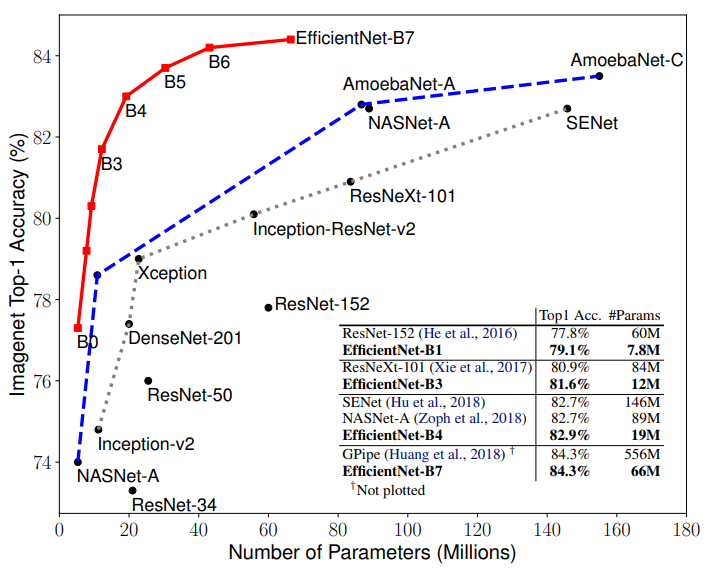
\includegraphics[width=0.8\linewidth]{images/efficientnet.PNG}
	\end{center}
	\caption{Comparison of EfficientNet to other state-of-the-art architectures on ImageNet (top-1 accuracy) compared to the number of parameters used}
	\label{fig:efficientnet}
\end{figure}

\autoref{fig:efficientnet} shows a 84.3\% top-1 accuracy score of EfficientNet-B7 on ImageNet outperforming other networks like ResNet or DenseNet while at the same time having far fewer parameters to train. \cite{LeMingxingTan.2019}

All these recent achievements on CNNs were based on manual architecture search. As opposed to such manual search, neural architecture search (NAS) tries to automate the process of finding suitable network architectures by applying a policy-gradient based reinforcement learning method over a specified design space. A RNN therefore continuously creates new network architectures which get evaluated on a target dataset. The achieved accuracy is then fed back as a reward signal to the RNN. \cite{LeBarretZoph.2017}

In \cite{BarretZoph.2018} this NAS is first performed on the small CIFAR-10 dataset in order to efficiently find a suitable architecture for a single convolutional cell. The design space used is called NASNet. The resulting cell architecture is then stacked to an entire CNN to perform image classification on the larger ImageNet dataset. Each convolutional cell has the same architecture but different weights. NASNet achieves a 2.4\% error rate on CIFAR-10 and a 82.7\% top-1 accuracy, resp. 96.2\% top-5 accuracy on ImageNet while having 28\% less computational complexity. 

This method was lateron outperformed by \cite{ChenxiLiu.2018} which uses a heuristic search to find suitable convolutional cells and a surrogate function to predict its performance to limit the amount of convolutional cells to train. It is five times more efficient regarding the number of models evaluated and eight times faster regarding the total computational effort than \cite{BarretZoph.2018}. 

Besides reinforcement learning methods there is also an evolutionary algorithms approach to neural architecture search with comparable results in model accuracy \cite{EstebanReal.2019}.

One layer of abstraction higher, one can also search for suitable design spaces in order to derive a common understanding about important design principles. RegNet is such a design space derived from AnyNet, the largest possible design space without further constraints, by iteratively parametrizing whole populations of diverse networks and searching for the simplest but most perfomant population. Using this technique one can iteratively eliminate design space dimensions that are actually not too important for the network design because of similar perfomances. For instance, using a bootleneck compression ratio does not influence model performance and could thus be excluded from the design space by making it a static constraint. Increasing the depth or width of networks on the other hand is one of the key design space dimensions. The resulting population of RegNet was able to outperform EfficientNet. \cite{IlijaRadosavovic.2020}

There are some other achitecture worth mentioning, one of them being Xception. It uses so-called depthwise separable convolutional layers, which are similar to the  multi-branch architectural Inception componenets from GooLeNet, but first convolutes spatially and afterwards convolutes the resulting channels using 1x1 convolutional layers (pointwise convolution) without using non-linearity components in between. It therefore maps spatial and cross-channel correlations completely separately. The Xception architecture is a linear stack of depthwise separable convolution layers with residual connections, but only achieves negligible improvements on its competitor Inceptionv3 on ImageNet. \cite{FrancoisChollet.2017}

MobileNet takes use of such depthwise separable convolutional layers in their nature of data reduction in order to make CNNs accessible for mobile and embedded systems. It furthermore introduces two more hyperparameters, a width multiplier and resolution multiplier, to better trade-off between speed and accuracy (respectively latency and size). The width multiplier is multiplied with the input and output channels of each layer thus reducing the computational costs and number of parameters quadratically. Same goes for the resolution multiplier that is applied to the input image and subsequent layers. 95\% of the computation time and 75\% of the parameters of such MobileNets can be traced back to the pointwise 1x1 convolutions. In terms of accuracy MobileNet can be compared to VGG16 while being 32 times smaller and 27 times less computationally expensive (measured by the Mult Adds). \cite{AndrewGHoward.2017}

ShuffleNet designed for mobile devices also builds upon depthwise separable convolutional layers and combines it with pointwise group convolution to gain additional speed through reducing computational expenses in a novel way. Possible information bottlenecks by the pointwise group convolution are tackled by using subsequent channel shuffeling to keep the information flow entropy of channels the same. ShuffleNet outperforms MobileNet by having a 7.8\% lower ImageNet top-1 error at level of 40 MFLOPs, but also having 32 layers more than the original MobileNet. Nevertheless succeeding experiments reduced depth still showed a superior behavior. \cite{XiangyuZhang.2017}

The next evolutionary step of ShuffleNet was made compliant to several design principles derived to optimize general model behavior. Oftentimes the indirect metric of FLOPS as a measure for computational complexity is taken to derive speed quality guarantees of a network. Nevertheless, the direct metric speed is influenced by far more parameters than just FLOPS like memory access costs (MAC), the degree of parallelism and the optimized runtime of the target platform making FLOPS as a solely metric insufficient. FLOPS are take account for convolutional operations, but I/O operations, data shuffling or element-wise operations also are not be be neglected. The authors derive four design principles by which the original ShuffleNet architecture was revised beating its predecessor and MobileNet v2: \cite{NingningMa.2018}

\begin{itemize}
	\item equal channel width minimizes memory access cost, 
	\item excessive group convolution increases MAC, 
	\item network fragmentation reduces degree of parallelism and
	\item element-wise operations are non-negligible
\end{itemize}

After these evolutionary steps of CNNs, the question arises whether it really needs such huge and complicated architectures to train a decent model or whether simple models can achieve comparable results. 

\cite{LechaoXiao.2018} gives a proof that plain CNNs with huge depths (10k layers) can be trained to give reasonable results (99\% test accuracy on MNIST and 82\% on CIFAR-10). Therefore a theoretical framework built upon mean field theory guided the design of an initialization scheme (delta-orthogonal initialization) that enables signals to smoothly flow through the entire network without being slowly reduced. 

\cite{OyebadeOyedotun.2020} is another paper giving proof of well performing deep plain CNNs. It uses LReLU to tackle the units' activations saturation/explosion and max-norm constraint on the weights to prevent exploding gradients. Also a strategic parameter initialization scheme is introduced. Using this approach plain CNNs of up to 100 layers can be trained sufficiently well. On ImageNet the best performing plain CNN was 30 layers deep giving a top-1 error of 24.1\% and a top-5 error of 7.3\%, slightly better than VGG-19 with comparable parameter size. 

\cite{SergeyZagoruyko.2018} with its novel Dirac weight parameterization given by the equation 

\begin{equation}
	\hat{W} = diag(a)I + diag(b)W_{norm}
\end{equation}

with $a$ and $b$ being scaling vectors learned during training and $W_{norm}$ being a normalized weight vector, introduces a way to achieve deep network performances close to residual networks without actual skip-connections. Having a closer look one recognizes that the Dirac weight parameterization and residual networks approximately only differ in the order of non-linearities:

\begin{equation}
	y = \sigma((diag(a)I + diag(b)W_{norm}) X) \approx \sigma(X + W'X)
\end{equation}

\begin{equation}
	y = X + \sigma(WX)
\end{equation}

During the experiments, DiracNet was able to outperform other plain networks that did not manage to converge anymore after a 100-layer depth. Also DiracNet was able to closely match 1001-layer ResNet with only 28 layers on CIFAR-10 as well as ResNet-18 and ResNet-34 on ImageNet wile having the same amount of parameters (27.79\% vs. 27.17\% top-1 error with 34-layer depth configuration). 

Another structural re-parameterization technique is given by the asymmetric convolutional block (ACB) from \cite{XiaohanDing.2019}. During training time a normal squared 3x3 convolutional kernel is replaced by multi-branch 3x3, 3x1 and 1x3 kernels that are added back together after batch-normalization. ACBs are architecture-neutral meaning can can replace normal 3x3 conv layers without having additional hyperparameters to tune, without further assumptions to take about the model and without additional computational complexity induced. For inference time these asymmetric kernels are added on top of each other forming again conventional 3x3 convolutional kernels initialized with the converted learned parameters. This re-parameterization technique strengthens the skeletons of squared convolutional kernels (that are naturally of higher magnitude), but in practice only leads to few but consistent performance improvements.  

Further re-parameterization techniques are DO-Conv (depthwise over-parameterized) layers \cite{JinmingCao.2020} and additional consecutive linear layers without further non-linearity in between by ExpandNet \cite{ShuxuanGuo.2021}. Note that both architectures just like ACBs can also be folded back into the same structure as the original for the inference time. 

Now after reducing the complexity of a network by studies of plain convolutional nets and re-parameterization techniques, one can also optimize the running time of convolutional nets by optimizing the actual computation technique. Winograd convolution offers such a fast algorithms to calculate small 3x3 convolutions with stride one on small batch sizes. Imagine a one-dimensional example of a filter size of 3 and output size 2:

\begin{figure}[ht]
	\begin{center}
		% \fbox{\rule{0pt}{2in}\rule{0.9\linewidth}{0pt}}
		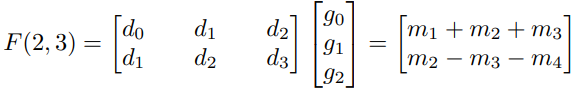
\includegraphics[width=0.8\linewidth]{images/winograd1.PNG}
	\end{center}
	\label{fig:winograd1}
\end{figure}

\begin{figure}[ht]
	\begin{center}
		% \fbox{\rule{0pt}{2in}\rule{0.9\linewidth}{0pt}}
		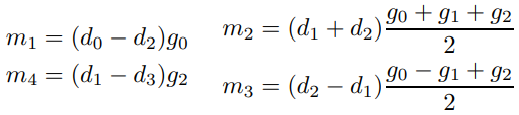
\includegraphics[width=0.8\linewidth]{images/winograd2.PNG}
	\end{center}
	\label{fig:winograd2}
\end{figure}

Using this method the 6 MULs from original convolution can be reduced to just 4 MULs. Generalizing this to two-dimensional kernels and inputs in the spacial dimension, channels and multiple filters, the arithmetic complexity can still be reduced up to a factor of 4 compared to direct convolution. This optimization is based on reducing the amount of duplication when applying kernels using a sliding window approach. It reduces the amount of computation by reducing duplication and is therefore also much more cache-efficient. \cite{AndrewLavin.2015}